\subsection{实验环境与设置}
环境用 PyTorch 在 GPU 上批量并行实现，所有人的感知、移动、碰撞和抓捕都写成张量运算，在一块 NVIDIA RTX 4070 Laptop GPU（8 GB）上运行，软件环境为 Python 3.12 与 PyTorch。

实验分四部分，一轮都是 30 分钟。脚本策略实验每种条件跑 256 局，同一局里 20 只老鼠按五种策略各 4 只分配，用局内配对比较。“哪里最好躲”实验让每只老鼠开局被分到全图随机的一个藏身点，共 2 × 256 局。上下两轮转化实验对 5 种躲的比例各跑 256 局。共同训练实验有八组：猫的五种奖励（个人、团队、混合、按参与分配、随机分配）、隐蔽无优势、历史对手池、只用最新对手。每组 3 个种子，普通组训练 300 轮（每个约 27 分钟），对手池两组训练 600 轮（每个约 50 分钟），之后每个种子用 64 局做交叉评估。在上真实地图之前，笔者先在 50 m × 50 m 的抽象小场地上做了一轮机制探针，结果见第~\ref{sec:res-probe} 节。

\subsection{先导实验：小场地上，躲赢在“动起来更显眼”}
\label{sec:res-probe}
小场地上扫了四个因素：掩体多少、体力是否有限、静止时是否更难被发现、老鼠知不知道谁刚变成猫，每种条件跑 1024 局，一局 300 s。如图~\ref{fig:probe}a，只要“动静一样显眼”，躲就不比跑好，体力无限时在空地上跑反而多活 10 s；一旦静止时更难被发现，躲在每种掩体数量下都赢。体力限制的作用比预想的小。小场地上没有灌木和夹缝这样的“难被看见的地形”，所以这里只检验了“静止”这一项。

\begin{figure}[htbp]
  \centering
  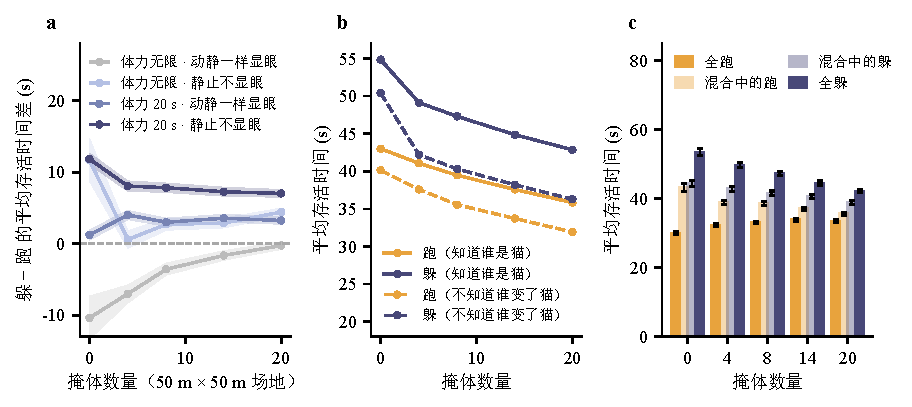
\includegraphics[width=\textwidth]{fig1_hide_vs_run.pdf}
  \caption{\figlead{在 50 m 小场地上，只有“动起来更显眼”时，躲才稳定地比跑活得久。}
  \textbf{a}，同一局里躲的老鼠减去跑的老鼠的平均存活时间差，按四种“体力 × 显眼度”组合画出。阴影为 95\% 自举区间，每点 1024 局。
  \textbf{b}，老鼠不知道谁刚变成猫时（虚线），躲的优势缩小。
  \textbf{c}，体力 20 s、动静一样显眼时，全跑、全躲和混合（各半）三种群体下的人均存活。误差棒为 95\% 自举区间。}
  \label{fig:probe}
\end{figure}

笔者也在小场地上训练了只有老鼠学习的 PPO（猫是脚本，每种条件 3 个种子，图~\ref{fig:probe-ppo}）。在真实条件下，AI 老鼠活 51–56 s，比脚本躲（50 s）和脚本跑（39 s）都久。它学到的不是“躲到掩体后面”：只有 6\% 的时间贴着掩体，却有 70\% 的时间贴着墙。背靠墙，危险只会从半边来。

\begin{figure}[htbp]
  \centering
  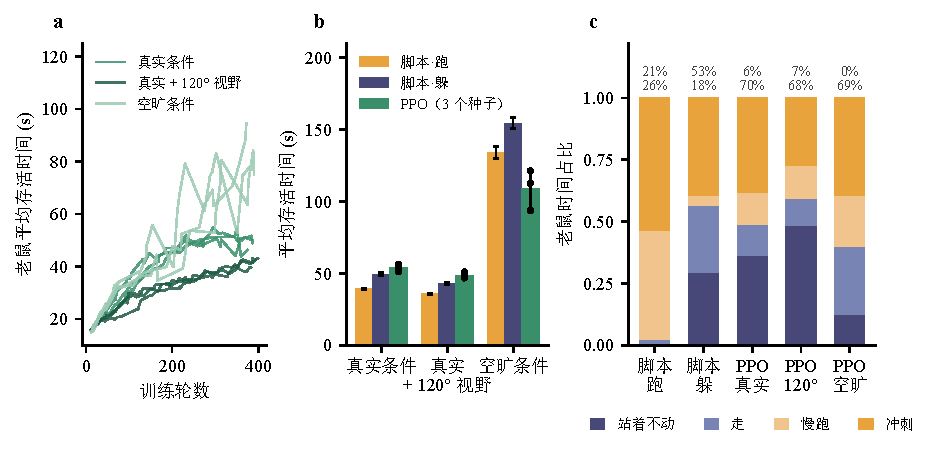
\includegraphics[width=\textwidth]{fig2_ppo_behavior.pdf}
  \caption{\figlead{小场地上的 AI 老鼠学会了“背靠墙站着不动”，而不是躲到掩体后面。}
  \textbf{a}，训练曲线，每条线一个随机种子。
  \textbf{b}，评估时的平均存活时间，评估用训练时没见过的地图布局。脚本策略的误差棒为 95\% 自举区间；PPO 的黑点是各种子的结果，误差棒为 3 个种子的最小值到最大值。
  \textbf{c}，老鼠时间分配。柱顶两行数字分别是贴掩体、贴墙的时间占比。}
  \label{fig:probe-ppo}
\end{figure}
